\begin{figure*}[t]
    \centering
    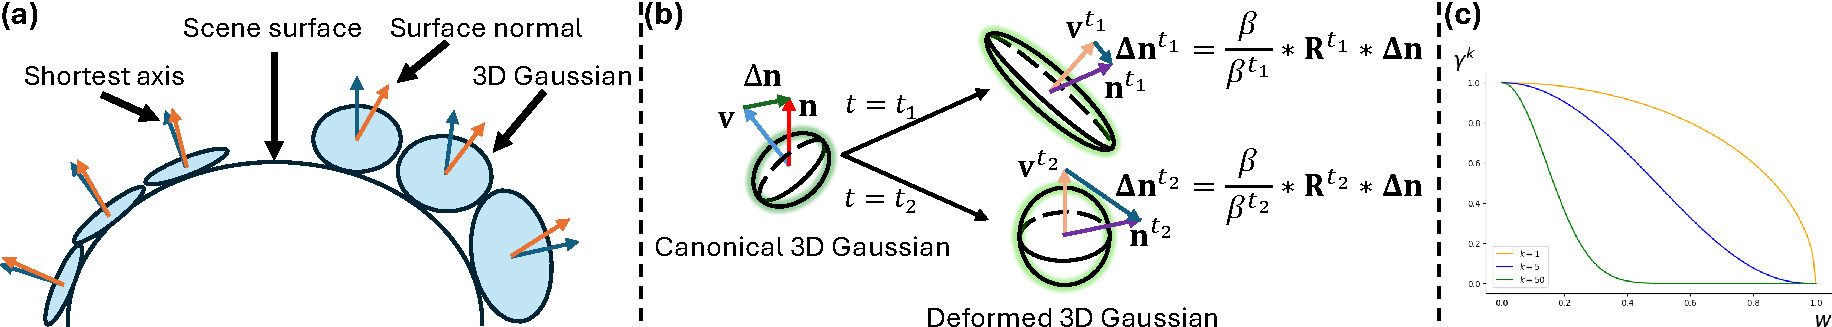
\includegraphics[width=1\linewidth]{figures/normal.pdf}
    \caption{\textbf{Normal estimation.} \textbf{(a)} shows that flatter 3D Gaussians align better with scene surfaces, their shortest axis closely matching the surface normal. In contrast, less flat 3D Gaussians fit less accurately, with their shortest axis diverging from the surface normal. \textbf{(b)} shows that when the deformed 3D Gaussian becomes flatter ($t=t_1$),  normal residual $\Delta\mathbf{n}$ is rotated by $\mathbf{R}^t_1$ and scaled down by $\frac{\beta}{\beta^t_1}$, as flatter Gaussians require smaller normal residuals. Conversely, when the deformation results in a less flat shape ($t=t_2$), $\Delta\mathbf{n}$ is rotated by $\mathbf{R}^t_2$ and amplified by $\frac{\beta}{\beta^t_2}$, requiring a larger correction to align the shortest axis with the surface normal. \textbf{(c)} shows how $\gamma^k$ changes with $w$ (where $w = \frac{|\mathbf{v}_s^t|}{|\mathbf{v}_l^t|}$) for $k=1$, $k=5$, and $k=50$. Larger $w$ indicates less flat Gaussians, while smaller $w$ represents flatter Gaussians. As $k$ increases, $\gamma^k$ decreases more steeply as $w$ rises. For $k=5$, we observe a balanced behavior: $\gamma^k$ approaches 1 for low $w$ and 0 for high $w$, providing a nuanced penalty adjustment across different Gaussian shapes.}
    \label{fig:normal_estimation}
\end{figure*}